\documentclass[journal,12pt,twocolumn]{IEEEtran}

\usepackage{setspace}
\usepackage{gensymb}

\singlespacing


\usepackage[cmex10]{amsmath}

\usepackage{amsthm}

\usepackage{mathrsfs}
\usepackage{txfonts}
\usepackage{stfloats}
\usepackage{bm}
\usepackage{cite}
\usepackage{cases}
\usepackage{subfig}

\usepackage{longtable}
\usepackage{multirow}

\usepackage{enumitem}
\usepackage{mathtools}
\usepackage{steinmetz}
\usepackage{tikz}
\usepackage{circuitikz}
\usepackage{verbatim}
\usepackage{tfrupee}
\usepackage[breaklinks=true]{hyperref}
\usepackage{graphicx}
\usepackage{tkz-euclide}
\usepackage{float}

\usetikzlibrary{calc,math}
\usepackage{listings}
    \usepackage{color}                                            %%
    \usepackage{array}                                            %%
    \usepackage{longtable}                                        %%
    \usepackage{calc}                                             %%
    \usepackage{multirow}                                         %%
    \usepackage{hhline}                                           %%
    \usepackage{ifthen}                                           %%
    \usepackage{lscape}     
\usepackage{multicol}
\usepackage{chngcntr}

\DeclareMathOperator*{\Res}{Res}

\renewcommand\thesection{\arabic{section}}
\renewcommand\thesubsection{\thesection.\arabic{subsection}}
\renewcommand\thesubsubsection{\thesubsection.\arabic{subsubsection}}

\renewcommand\thesectiondis{\arabic{section}}
\renewcommand\thesubsectiondis{\thesectiondis.\arabic{subsection}}
\renewcommand\thesubsubsectiondis{\thesubsectiondis.\arabic{subsubsection}}


\hyphenation{op-tical net-works semi-conduc-tor}
\def\inputGnumericTable{}                                 %%

\lstset{
%language=C,
frame=single, 
breaklines=true,
columns=fullflexible
}
\begin{document}


\newtheorem{theorem}{Theorem}[section]
\newtheorem{problem}{Problem}
\newtheorem{proposition}{Proposition}[section]
\newtheorem{lemma}{Lemma}[section]
\newtheorem{corollary}[theorem]{Corollary}
\newtheorem{example}{Example}[section]
\newtheorem{definition}[problem]{Definition}

\newcommand{\BEQA}{\begin{eqnarray}}
\newcommand{\EEQA}{\end{eqnarray}}
\newcommand{\define}{\stackrel{\triangle}{=}}
\newcommand\hlight[1]{\tikz[overlay, remember picture,baseline=-\the\dimexpr\fontdimen22\textfont2\relax]\node[rectangle,fill=blue!50,rounded corners,fill opacity = 0.2,draw,thick,text opacity =1] {$#1$};}
\bibliographystyle{IEEEtran}
\providecommand{\mbf}{\mathbf}
\providecommand{\pr}[1]{\ensuremath{\Pr\left(#1\right)}}
\providecommand{\qfunc}[1]{\ensuremath{Q\left(#1\right)}}
\providecommand{\sbrak}[1]{\ensuremath{{}\left[#1\right]}}
\providecommand{\lsbrak}[1]{\ensuremath{{}\left[#1\right.}}
\providecommand{\rsbrak}[1]{\ensuremath{{}\left.#1\right]}}
\providecommand{\brak}[1]{\ensuremath{\left(#1\right)}}
\providecommand{\lbrak}[1]{\ensuremath{\left(#1\right.}}
\providecommand{\rbrak}[1]{\ensuremath{\left.#1\right)}}
\providecommand{\cbrak}[1]{\ensuremath{\left\{#1\right\}}}
\providecommand{\lcbrak}[1]{\ensuremath{\left\{#1\right.}}
\providecommand{\rcbrak}[1]{\ensuremath{\left.#1\right\}}}
\theoremstyle{remark}
\newtheorem{rem}{Remark}
\newcommand{\sgn}{\mathop{\mathrm{sgn}}}
\providecommand{\abs}[1]{\left\vert#1\right\vert}
\providecommand{\res}[1]{\Res\displaylimits_{#1}} 
\providecommand{\norm}[1]{\left\lVert#1\right\rVert}
%\providecommand{\norm}[1]{\lVert#1\rVert}
\providecommand{\mtx}[1]{\mathbf{#1}}
\providecommand{\mean}[1]{E\left[ #1 \right]}
\providecommand{\fourier}{\overset{\mathcal{F}}{ \rightleftharpoons}}
%\providecommand{\hilbert}{\overset{\mathcal{H}}{ \rightleftharpoons}}
\providecommand{\system}{\overset{\mathcal{H}}{ \longleftrightarrow}}
	%\newcommand{\solution}[2]{\textbf{Solution:}{#1}}
\newcommand{\solution}{\noindent \textbf{Solution: }}
\newcommand{\cosec}{\,\text{cosec}\,}
\providecommand{\dec}[2]{\ensuremath{\overset{#1}{\underset{#2}{\gtrless}}}}
\newcommand{\myvec}[1]{\ensuremath{\begin{pmatrix}#1\end{pmatrix}}}
\newcommand{\mydet}[1]{\ensuremath{\begin{vmatrix}#1\end{vmatrix}}}
\numberwithin{equation}{subsection}
\makeatletter
\@addtoreset{figure}{problem}
\makeatother
\let\StandardTheFigure\thefigure
\let\vec\mathbf
\renewcommand{\thefigure}{\theproblem}
\def\putbox#1#2#3{\makebox[0in][l]{\makebox[#1][l]{}\raisebox{\baselineskip}[0in][0in]{\raisebox{#2}[0in][0in]{#3}}}}
     \def\rightbox#1{\makebox[0in][r]{#1}}
     \def\centbox#1{\makebox[0in]{#1}}
     \def\topbox#1{\raisebox{-\baselineskip}[0in][0in]{#1}}
     \def\midbox#1{\raisebox{-0.5\baselineskip}[0in][0in]{#1}}
\vspace{3cm}
\title{Assignment 12}
\author{K.A. Raja Babu}
\maketitle
\newpage
\bigskip
\renewcommand{\thefigure}{\theenumi}
\renewcommand{\thetable}{\theenumi}
Download all python codes from 
\begin{lstlisting}
https://github.com/ka-raja-babu/Matrix-Theory/tree/main/Assignment12/Codes
\end{lstlisting}
%
and latex-tikz codes from 
%
\begin{lstlisting}
https://github.com/ka-raja-babu/Matrix-Theory/tree/main/Assignment12
\end{lstlisting}
%
\section{Question No. 2.36}

\textbf{(Diet problem)} A dietician has to develop a special diet using two foods P and Q. Each packet (containing 30 g) of food P contains 12 units of calcium, 4 units of iron, 6 units of cholesterol and 6 units of vitamin A. Each packet of the same quantity of food Q contains 3 units of calcium, 20 units of iron, 4 units of cholesterol and 3 units of vitamin A. The diet requires at least 240 units of calcium, at least 460 units of iron and at most 300 units of cholesterol. How many packets of each food should be used to minimise the amount of vitamin A in the diet ? What is the minimum amount of vitamin A ?

\section{Solution}

\numberwithin{table}{section}
\begin{table}[!ht]
\begin{center}
\begin{tabular}{ | m{2.1cm} | m{1.4cm}| m{1.4cm} | m{2.2cm} | } 
\hline
Component & P & Q & Requirement \\
\hline
Calcium & 12 units & 3 units & $\geq 240$ units \\ 
\hline
Iron & 4 units & 20 units & $\geq 460$ units \\ 
\hline
Cholesterol & 6 units & 4 units & $\leq 300$ units\\ 
\hline
Vitamin A & 6 units & 3 units & \\ 
\hline
\end{tabular}
\end{center}
\caption{Diet Requirements}
\label{tab:table1}
\end{table}

Let the number of packets of food P be $x$ and the number of packets of food Q be $y$  such that 
\begin{align}
    x \geq 0 \\
    y \geq 0 
\end{align}

According to the question,
\begin{align}
    12x+3y &\geq 240 \\
    \implies -4x-y &\leq -80 \\
\end{align}
and,
\begin{align}
    4x+20y &\geq 460 \\
    \implies -x-5y &\leq -115 
\end{align}
and,
\begin{align}
     6x+4y &\leq 300 \\
    \implies 3x+2y &\leq 150 \\
\end{align}

$\therefore$ Our problem is
\begin{align}
    \text{Minimize}:Z &= 6x+3y\\
    \text{Subject to}:
    -4x-y &\leq -80  \label{con1} \\
    -x-5y &\leq -115 \label{con2} \\
    3x+2y &\leq 150 \\
    -x &\leq 0 \\
    -y &\leq 0
\end{align}

Lagrangian function is given by
\begin{equation}
\begin{aligned}
    L(\vec{x},\lambda) &= (6x+3y)+(-4x-y+80)\lambda_1 \\ &+ (-x-6y+115)\lambda_2 +(3x+2y-150)\lambda_3 \\ &- x\lambda_4 -y\lambda_5
\end{aligned}
\end{equation}

Now,
\begin{align}
    \nabla L(\vec{x},\lambda) &= \myvec{6-4\lambda_1-\lambda_2+3\lambda_3-\lambda_4 \\ 3-\lambda_1-5\lambda_2+2\lambda_3-\lambda_5 \\ -4x-y+80 \\ -x-5y+115 \\ 3x+2y-150 \\ -x \\ -y}
\end{align}

$\therefore$ Lagrangian matrix is given by
\begin{align}
    \myvec{0 & 0 & -4 & -1 & 3 & -1 & 0 \\ 0 & 0 & -1 & -5 & 2 & 0 & -1 \\ -4 & -1 & 0 & 0 & 0 & 0 & 0 \\ -1 & -5 & 0 & 0 & 0 & 0 & 0 \\ 3 & 2 & 0 & 0 & 0 & 0 & 0 \\ -1 & 0 & 0 & 0 & 0 & 0 & 0 \\ 0 & -1 & 0 & 0 & 0 & 0 & 0 }\myvec{x \\ y \\ \lambda_1 \\ \lambda_2 \\ \lambda_3 \\ \lambda_4 \\ \lambda_5 } &= \myvec{-6 \\ -3 \\ -80 \\ -115 \\ 150 \\ 0 \\0 }
\end{align}
Considering eq.\eqref{con1} and eq.\eqref{con2} as only active constraints,
\begin{align}
    \myvec{0 & 0 & -4 & -1 \\ 0 & 0 & -1 & -5 \\ -4 & -1 & 0 & 0 \\ -1 & -5 & 0 & 0}\myvec{x \\ y \\ \lambda_1 \\ \lambda_2} &= \myvec{-6 \\ -3 \\ -80 \\ -115}
\end{align}
resulting in,
\begin{align}
    \myvec{x \\ y \\ \lambda_1 \\ \lambda_2} &= \myvec{0 & 0 & -4 & -1 \\ 0 & 0 & -1 & -5 \\ -4 & -1 & 0 & 0 \\ -1 & -5 & 0 & 0}^{-1}\myvec{-6 \\ -3 \\ -80 \\ -115}
    \\
    \implies   \myvec{x \\ y \\ \lambda_1 \\ \lambda_2} &= \myvec{0 & 0 & \frac{-5}{19} & \frac{1}{19} \\ 0 & 0 & \frac{1}{19} & \frac{-4}{19} \\ \frac{-5}{19} & \frac{1}{19} & 0 & 0 \\ \frac{1}{19} & \frac{-4}{19} & 0 & 0}\myvec{-6 \\ -3 \\ -80 \\ -115}
    \\
    \implies \myvec{x \\ y \\ \lambda_1 \\ \lambda_2 } &= \myvec{15 \\ 20 \\ \frac{27}{19} \\ \frac{6}{19} }
\end{align}
$\because \lambda_1,\lambda_2 > 0 $
\\
$\therefore$ Optimal solution is given by
\begin{align}
    x &= 15 \\
    y &= 20 \\
    Z &= 6x+3y \\
    &= 6(15) + 3(20) \\
    &= 150
\end{align}
Problem can also be represented in matrix form as
\begin{align}
        \min_{\vec{x}} Z &= \myvec{6 & 3}\vec{x}\\
        s.t. \quad 
        \myvec{4 & 1 \\ 1 & 5 \\ -3 & -2 }\vec{x} &\succeq \myvec{80\\115\\-150} \\
        \vec{x} &\succeq \vec{0}
    \end{align}
    
By using cvxpy in python ,
\begin{align}
    \vec{x}=\myvec{14.99999999\\20.00000001}\\
    Z = 150.00000001
\end{align}

Hence ,\boxed{x=15} packets of food P and \boxed{y=20} packets of food Q should be used to minimise the amount of vitamin A in the diet and the minimum amount of vitamin A is \boxed{Z=150} units .

\numberwithin{figure}{section}
\begin{figure}[!ht]
\centering
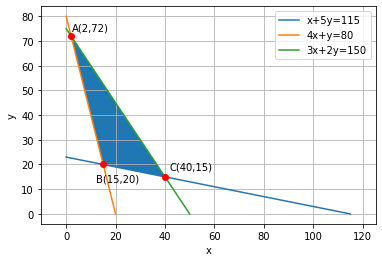
\includegraphics[width=\columnwidth]{Figure12}
\caption{Diet Problem}
\label{fig:diet problem}	
\end{figure}

\end{document}

